% Options for packages loaded elsewhere
\PassOptionsToPackage{unicode}{hyperref}
\PassOptionsToPackage{hyphens}{url}
%
\documentclass[
]{book}
\usepackage{amsmath,amssymb}
\usepackage{lmodern}
\usepackage{ifxetex,ifluatex}
\ifnum 0\ifxetex 1\fi\ifluatex 1\fi=0 % if pdftex
  \usepackage[T1]{fontenc}
  \usepackage[utf8]{inputenc}
  \usepackage{textcomp} % provide euro and other symbols
\else % if luatex or xetex
  \usepackage{unicode-math}
  \defaultfontfeatures{Scale=MatchLowercase}
  \defaultfontfeatures[\rmfamily]{Ligatures=TeX,Scale=1}
\fi
% Use upquote if available, for straight quotes in verbatim environments
\IfFileExists{upquote.sty}{\usepackage{upquote}}{}
\IfFileExists{microtype.sty}{% use microtype if available
  \usepackage[]{microtype}
  \UseMicrotypeSet[protrusion]{basicmath} % disable protrusion for tt fonts
}{}
\makeatletter
\@ifundefined{KOMAClassName}{% if non-KOMA class
  \IfFileExists{parskip.sty}{%
    \usepackage{parskip}
  }{% else
    \setlength{\parindent}{0pt}
    \setlength{\parskip}{6pt plus 2pt minus 1pt}}
}{% if KOMA class
  \KOMAoptions{parskip=half}}
\makeatother
\usepackage{xcolor}
\IfFileExists{xurl.sty}{\usepackage{xurl}}{} % add URL line breaks if available
\IfFileExists{bookmark.sty}{\usepackage{bookmark}}{\usepackage{hyperref}}
\hypersetup{
  pdftitle={Synthesis},
  pdfauthor={Dyrehaugen Web Notebook},
  hidelinks,
  pdfcreator={LaTeX via pandoc}}
\urlstyle{same} % disable monospaced font for URLs
\usepackage{longtable,booktabs,array}
\usepackage{calc} % for calculating minipage widths
% Correct order of tables after \paragraph or \subparagraph
\usepackage{etoolbox}
\makeatletter
\patchcmd\longtable{\par}{\if@noskipsec\mbox{}\fi\par}{}{}
\makeatother
% Allow footnotes in longtable head/foot
\IfFileExists{footnotehyper.sty}{\usepackage{footnotehyper}}{\usepackage{footnote}}
\makesavenoteenv{longtable}
\usepackage{graphicx}
\makeatletter
\def\maxwidth{\ifdim\Gin@nat@width>\linewidth\linewidth\else\Gin@nat@width\fi}
\def\maxheight{\ifdim\Gin@nat@height>\textheight\textheight\else\Gin@nat@height\fi}
\makeatother
% Scale images if necessary, so that they will not overflow the page
% margins by default, and it is still possible to overwrite the defaults
% using explicit options in \includegraphics[width, height, ...]{}
\setkeys{Gin}{width=\maxwidth,height=\maxheight,keepaspectratio}
% Set default figure placement to htbp
\makeatletter
\def\fps@figure{htbp}
\makeatother
\setlength{\emergencystretch}{3em} % prevent overfull lines
\providecommand{\tightlist}{%
  \setlength{\itemsep}{0pt}\setlength{\parskip}{0pt}}
\setcounter{secnumdepth}{5}
\usepackage{booktabs}
\usepackage{amsthm}
\makeatletter
\def\thm@space@setup{%
  \thm@preskip=8pt plus 2pt minus 4pt
  \thm@postskip=\thm@preskip
}
\makeatother

\renewcommand\chaptername{}
\ifluatex
  \usepackage{selnolig}  % disable illegal ligatures
\fi
\usepackage[]{natbib}
\bibliographystyle{apalike}

\title{Synthesis}
\author{Dyrehaugen Web Notebook}
\date{2021-05-10}

\begin{document}
\maketitle

{
\setcounter{tocdepth}{1}
\tableofcontents
}
\hypertarget{synthesis}{%
\chapter{Synthesis}\label{synthesis}}

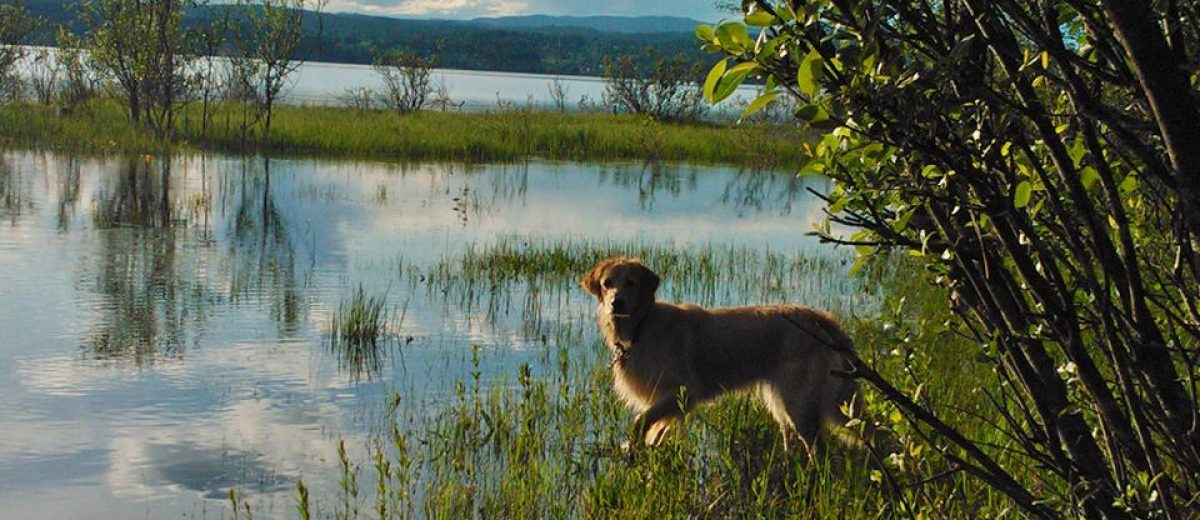
\includegraphics{fig/zelda.jpg}

\emph{Image: Zelda at Tyrefjorden}

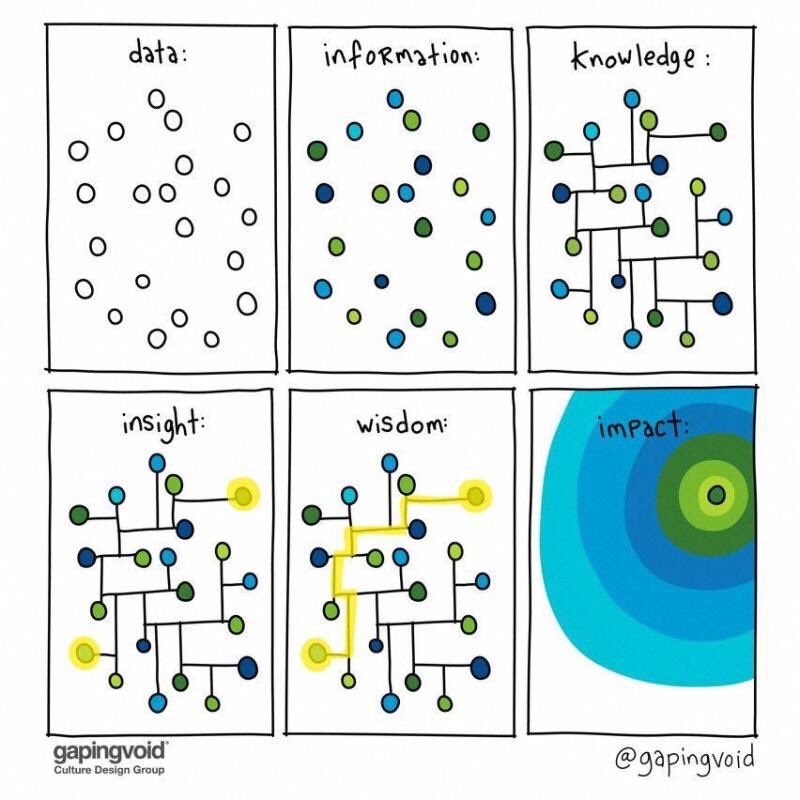
\includegraphics{fig/information_knowledge_2.jpeg}

\emph{Figure: Steps of Synthesis}

\hypertarget{capitalism}{%
\chapter{Capitalism}\label{capitalism}}

Background material can be found here: \href{https://dyrehaugen.github.io/rcap}{Dyrehaugen Notebook on Capitalism}\href{http://localhost/rcap}{(loc)}\footnote{\url{https://dyrehaugen.github.io/rcap}}

\hypertarget{overview}{%
\section{Overview}\label{overview}}

\emph{Pre-Capitalism}

\begin{verbatim}
Feudalism
Industrial Revolution
\end{verbatim}

\emph{Capitalism is a Legal Order}

\emph{Capitalism is Power}

\emph{Capitalism is Growth}

\emph{Capitalism is Plunder}

\emph{Capitalism is Fear}

\begin{verbatim}
Military Capitalism  
Derisking  
\end{verbatim}

\emph{Capitalism is Cancer}

\begin{verbatim}
Greenwashing Capitalism  
\end{verbatim}

\emph{Capitalism is Headless}

\begin{verbatim}
How to phase out Capitalism  
\end{verbatim}

\emph{Post-Capitalism}

\begin{verbatim}
Socialism for All, not just for The Rich
\end{verbatim}

\hypertarget{terminology}{%
\section{Terminology}\label{terminology}}

\emph{Capital - Wealth - Assets - Might} all translates in German into \emph{Vermögen}, even \emph{Kapitalvermögen}
- bringing the \emph{Power} aspect of \emph{Capital} into clear daylight.

\hypertarget{definition}{%
\section{Definition}\label{definition}}

Capitalism is the current Legal Order for Continous Accumulation of Wealth (Capital)
through Natural Resource Extraction, Labour Exploitation and Market Expansion (Trade).

\hypertarget{characteristics}{%
\section{Characteristics}\label{characteristics}}

\hypertarget{expansion}{%
\subsection{Expansion}\label{expansion}}

Capitalism is always expanding.
Its market system continues to annex new, previously uncommodified, realms.

\textbf{Outwards Expansion}

Colonialism - external trade - global value chains

\textbf{Inwards Expansion}

Commodification

\hypertarget{limited-liability}{%
\subsection{Limited Liability}\label{limited-liability}}

Corporations embrace new profit opportunities but rebuff the internalization of new costs.
As the decades go by, this ensures that the market, as an institution,
becomes ever more extractive or cost-shifting in nature.

\hypertarget{enabled-markets}{%
\subsection{Enabled Markets}\label{enabled-markets}}

We never have ``free markets.''
We only ever have ``enabled markets''

\hypertarget{state}{%
\subsection{State}\label{state}}

Markets are enabled by an authority - the State

\hypertarget{rule-of-law}{%
\subsection{Rule of Law}\label{rule-of-law}}

The State has to be capable of upholding the rule of law

\hypertarget{property}{%
\subsection{Property}\label{property}}

The Rule of Law is required to give Property meaning.

\hypertarget{commodification}{%
\subsection{Commodification}\label{commodification}}

Expansion by commodification - (privatising public services)

Technology creates opportunities for new commodifications -- and so make property of --
more and more.

\hypertarget{pre-capitalism}{%
\chapter{Pre-Capitalism}\label{pre-capitalism}}

\hypertarget{feudalism}{%
\section{Feudalism}\label{feudalism}}

\hypertarget{pre-industrial-capitalism}{%
\section{Pre-industrial Capitalism}\label{pre-industrial-capitalism}}

The new order of Capitalism emerged in the European burgs of the late Middle Ages.
It came as an reaction to the stagnation and violence of the feudaln régime.
It came with promise of dynamism, enlightenment (modern science) and prosperity.

Prior to the industrial turn wealth accumulated in commerce, mining and (simple)
manufacture.

A proto-capitalist was Jacob Fugger (1459-1525, Augsburg, Germany) who controlled
much of Europeean silver and copper production, turning this into \emph{monetized power}
as when paying for Charles V to become emperor of the Holy Roman Empire in 1519.

\hypertarget{slavery}{%
\section{Slavery}\label{slavery}}

Slavery were abandonned i Britain in 1834, in the US in 1864, in Brasil in 1888.
The proceeds from slavery formed the basis for the coming industrial revolution.

\hypertarget{industrial-revolution}{%
\section{Industrial Revolution}\label{industrial-revolution}}

\hypertarget{capitalism-is-a-legal-order}{%
\chapter{Capitalism is a Legal Order}\label{capitalism-is-a-legal-order}}

Capitalism is a socio-economic system structured through law.

At the base are the juridical concepts of

\begin{verbatim}
*equality (before the law)*
*freedom of contract*
*private property*
\end{verbatim}

The term ``capitalism'' became widespread in the late nineteenth century.
The earlier term was ``commercial society'' - for the regime of
material provision through market exchange.

\hypertarget{labour-law}{%
\section{Labour law}\label{labour-law}}

\hypertarget{corporate-law}{%
\section{Corporate law}\label{corporate-law}}

On September 24, 1599. In a timbered building off Moorgate Fields, not far from where Shakespeare was struggling to complete Hamlet, a new type of company was founded. Its ownership of the new firm, called the East India Company, was sliced into tiny pieces to be bought and sold freely.Tradable shares allowed private corporations to become larger and more powerful than states.

Corporate law empower corporations to make new property of new things that may be profitable for them -
(a modern example: everybody's internet activity).

Through lobbying and regulatory obstruction corporations have the power to prevent
new commodification of entities that would result in new costs (a modern example: CO2-price).

.

\hypertarget{competition-law}{%
\section{Competition law}\label{competition-law}}

\hypertarget{capitalism-is-power}{%
\chapter{Capitalism is Power}\label{capitalism-is-power}}

\hypertarget{capitalism-is-growth}{%
\chapter{Capitalism is Growth}\label{capitalism-is-growth}}

\hypertarget{capitalism-is-plunder}{%
\chapter{Capitalism is Plunder}\label{capitalism-is-plunder}}

The British Treasury only in 2015 finished paying off compensation
to slave owners for the abolishion of slavery in 1834.

\hypertarget{capitalism-is-fear}{%
\chapter{Capitalism is Fear}\label{capitalism-is-fear}}

\hypertarget{military-capitalism}{%
\section{Military Capitalism}\label{military-capitalism}}

\hypertarget{derisking}{%
\section{Derisking}\label{derisking}}

development scholars need to confront reality of a paradigm shift in development:

the rise of derisking as development strategy

bar UNCTAD, it has been embraced by every UN agency, MDBs, IMF, COP26 etc.

see 2021 report of Inter-Agency Task Force on Financing for Development

his is not just about Financing for Development, but aims to profoundly transform the state into risk-proofer for global finance

it has deep macrofinancial implications, involving monetary, fiscal and macropru, changing national development banks etc

(Daniela Gabor)

\hypertarget{capitalism-is-cancer}{%
\chapter{Capitalism is Cancer}\label{capitalism-is-cancer}}

\hypertarget{greenwashing-capitalism}{%
\section{Greenwashing Capitalism}\label{greenwashing-capitalism}}

\hypertarget{capitalism-is-headless}{%
\chapter{Capitalism is Headless}\label{capitalism-is-headless}}

Capitalism is `headless' - no one is in command of global development.

Capitalism develops historically in the direction of
`the resultant in the parallelogram of political forces'.

Global Development should not be `headless'.
We need a strategy to move beyond capitalism - to give Development a `mindful global head'.

\emph{Here are some ideas}.

\hypertarget{how-to-phase-out-capitalism}{%
\section{HOW TO PHASE OUT CAPITALISM}\label{how-to-phase-out-capitalism}}

\hypertarget{strategy}{%
\subsection{Strategy}\label{strategy}}

First turn extensive capitalism into intensive,
then let the intensive variant compete itself away (to monopoly = death of competition) !

\hypertarget{root-actions}{%
\subsection{Root Actions}\label{root-actions}}

\textbf{Scale back, Scale down, Degrow, Decellerate}

\begin{enumerate}
\def\labelenumi{(\arabic{enumi})}
\tightlist
\item
  Disallow limited liability
\item
  Disallow fractional credit
\item
  Disallow marketing - only independent information.
\item
  Disallow inheritance (100\% tax)
\item
  Disallow partial (not full life cycle) innovation
  (require food/medicine-like side-effects studies) (rquire system-wide recycling integration)
\item
  Disallow private land.
\item
  Disallow cross-trade
\item
  Flatten income and wealth distributions.
  Fat-tail focused economic policy Make wealth-statistics transparent. Plublish records for all of the
  fat tail. Refocus economic analysis from 'normal' middle to power-outliers
\item
  Reset economic system every 7th year (jubilee)
\item
  Disallow urban expansion.
\item
  Disallow un-wilding.
\item
  Disallow externalities (robbing the Commons).
\end{enumerate}

\hypertarget{actions-on-the-current-margin}{%
\subsection{Actions on the current margin}\label{actions-on-the-current-margin}}

\begin{enumerate}
\def\labelenumi{(\arabic{enumi})}
\item
  Next threat within the capitalistic logic: Establishment of Amazon in Scandinavia. How to unde-
  mind the trend? Linked to the precariate. Amazon should compensate locations which looses cur-
  rent shops - carry the costs of barnch restructurering. Monopolization fee.
\item
  Wind-Power industry degrading the landscape - we don't need more energy. Linked to land owner-
  ship - ownership of l!and does not contain the right to visual (and audio) polution ! Requirement:
  No-impact: Only invisible windmills allowed (i.e.:none)
\end{enumerate}

\hypertarget{reset-democracy}{%
\subsection{Reset Democracy}\label{reset-democracy}}

Lottery basaed representation - time limited.

\hypertarget{post-capitalism}{%
\chapter{Post Capitalism}\label{post-capitalism}}

\textbf{Many of the most important events haven't happened yet}

\hypertarget{socialism-for-all-not-just-for-the-rich}{%
\section{Socialism for All, not just for the Rich}\label{socialism-for-all-not-just-for-the-rich}}

\hypertarget{part-appendices}{%
\part{Appendices}\label{part-appendices}}

\hypertarget{appendix-appendices}{%
\appendix}


\hypertarget{about}{%
\chapter{About}\label{about}}

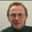
\includegraphics{fig/me.jpg}

\emph{Dyre Haugen} and \emph{Dyrehaugen} is Webian for \emph{Jon Martin} -
self-owned Globian, Webian, Norwegian and Canarian with
a background from industrial research policy, urban planning and
economic development consulting on global, regional and urban scales.
I am deeply concerned about the (insane) way
humanity (i.e.~capitalism) interfere with nature.
In an effort to gain insights in how and why this happens
stuff is collected from around the web and put together
in a linked set of web-sites.
The sites are operated as personal notebooks.
However, these days things can be easily published to the
benefit of others concerned with the same issues.
But be aware - this is not polished for presentation or
peer-reviewed for exactness.
I offer you just to have a look at my `work-desk' as it appears in the moment.
Any comment or suggestion can be mailed to \href{mailto:dyrehaugen@gmail.com}{\nolinkurl{dyrehaugen@gmail.com}}
You can follow me on twitter as @dyrehaugen.
Thanks for visiting!

\hypertarget{links}{%
\chapter{Links}\label{links}}

\textbf{Current Dyrehaugen Sites:}

\begin{itemize}
\tightlist
\item
  \href{https://dyrehaugen.github.io/rcap}{rcap - On Capitalism} \href{http://localhost/rcap}{(loc)}
\item
  \href{https://dyrehaugen.github.io/rclm}{rclm - On Climate Change} \href{http://localhost/rclm}{(loc)}
\item
  \href{https://dyrehaugen.github.io/recs}{recs - On Economics} \href{http://localhost/recs}{(loc)}
\item
  \href{https://dyrehaugen.github.io/rngy}{rfin - On Finance} \href{http://localhost/rfin}{(loc)}
\item
  \href{https://dyrehaugen.github.io/rngy}{rngy - On Energy} \href{http://localhost/rngy}{(loc)}
\item
  \href{https://dyrehaugen.github.io/renv}{renv - On Environment} \href{http://localhost/renv}{(loc)}
\item
  \href{https://dyrehaugen.github.io/rsts}{rsts - On Statistics} \href{http://localhost/rsts}{(loc)}
\item
  \href{https://dyrehaugen.github.io/rtch}{rtch - On Technology} \href{http://localhost/rtch}{(loc)}
\item
  \href{https://dyrehaugen.github.io/rurb}{rurb - On Urbanization} \href{http://localhost/rurb}{(loc)}
\item
  \href{https://dyrehaugen.github.io/rvar}{rvar - On Varia} \href{http://localhost/rvar}{(loc)}
\item
  \href{https://dyrehaugen.github.io/rwsd}{rwsd - On Wisdom} \href{http://localhost/rwsd}{(loc)}
\end{itemize}

\textbf{Blogs:}

\begin{itemize}
\tightlist
\item
  \href{https://dyrehaugen.github.io/rde}{rde - Blog in English} \href{http://localhost/rde}{(loc)}
\item
  \href{https://dyrehaugen.github.io/rdn}{rdn - Blog in Norwegian} \href{http://localhost/rdn}{(loc)}
\end{itemize}

\textbf{Discontinued:}

\begin{itemize}
\tightlist
\item
  \href{https://dyrehaugen.github.io/jdt}{jdt - Collection (Jekyll)} \href{http://localhost/jdt}{(loc)}
\item
  \href{https://dyrehaugen.github.io/hdt}{hdt - Collection (Hugo)} \href{http://localhost/hdt}{(loc)}
\end{itemize}

\textbf{Not listed:}

\begin{itemize}
\tightlist
\item
  (q:) dhe dhn jrw56
\item
  (z:) rcsa rpad rstart
\end{itemize}

\hypertarget{news}{%
\chapter{NEWS}\label{news}}

  \bibliography{book.bib,packages.bib}

\end{document}
